\documentclass{article}
% generated by Madoko, version 1.0.0-rc5
%mdk-data-line={1}


\usepackage[heading-base={2},section-num={False},bib-label={True}]{madoko2}


\begin{document}



%mdk-data-line={5}
\mdxtitleblockstart{}
%mdk-data-line={5}
\mdxtitle{\mdline{5}Optimization of the DNN program on the CPU+MIC Platform}%mdk
\mdxauthorstart{}
%mdk-data-line={10}
\mdxauthorname{\mdline{10}University of Electronic Secience and Technology of China}%mdk
\mdxauthorend\mdtitleauthorrunning{}{}\mdxtitleblockend%mdk

%mdk-data-line={6}
\section{\mdline{6}1.\hspace*{0.5em}\mdline{6}Preface}\label{sec-preface}%mdk%mdk

%mdk-data-line={7}
\noindent\mdline{7}In the section we are required to optimize a \mdline{7}\mdcode{DNN(deep~neural~network)}\mdline{7}
program based on a standalone hybrid CPU+MIC platform. The detailed
configuration is as follows:%mdk

%mdk-data-line={11}
\mdline{11}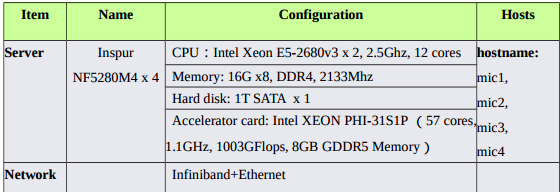
\includegraphics[keepaspectratio=true,width=\dimmin{}{\dimwidth{0.90}}]{images/2016-02-18-23-01-13-}{}\mdline{11}%mdk

%mdk-data-line={15}
\noindent\mdline{15}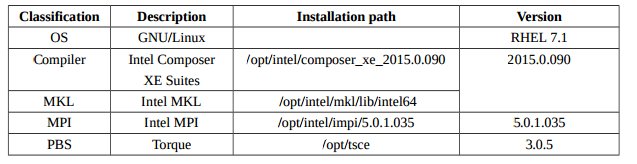
\includegraphics[keepaspectratio=true,width=\dimmin{}{\dimwidth{0.90}}]{images/2016-02-18-23-13-11-}{}\mdline{15}%mdk

%mdk-data-line={21}
\section{\mdline{21}2.\hspace*{0.5em}\mdline{21}Analysis of the serial program}\label{sec-analysis-of-the-serial-program}%mdk%mdk

%mdk-data-line={22}
\noindent\mdline{22}First, we generate a call graph by using \mdline{22}\mdcode{Google~perfools}\mdline{22},
 a open source performance profiler, to have a glance though it. Every
 square represents a function, and the bigger square is, the more time
 corresponding function cost.%mdk

%mdk-data-line={28}
\mdline{28}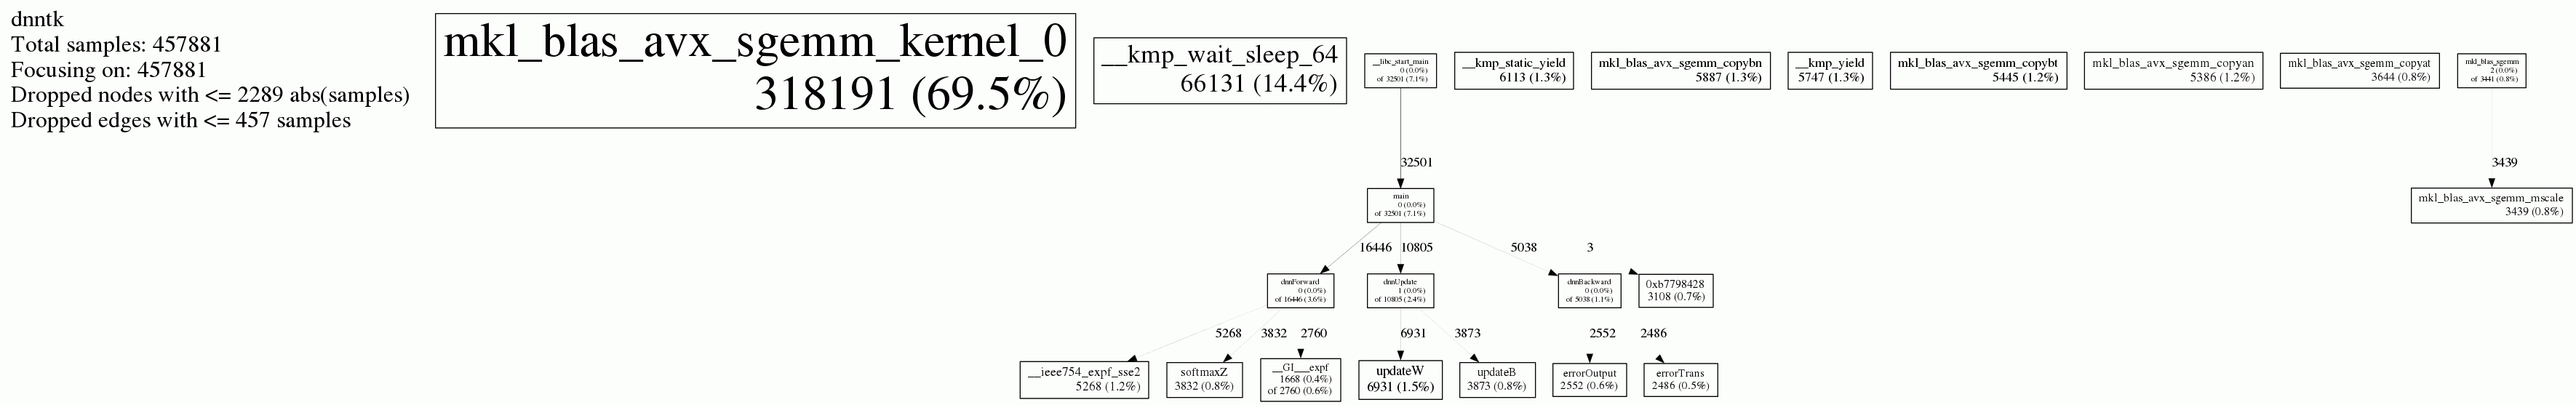
\includegraphics[keepaspectratio=true,width=\dimmin{}{\dimwidth{0.90}}]{images/100001994364201}{}\mdline{28}%mdk

%mdk-data-line={32}
\noindent\mdline{32}Obviously, the hot spot is something about \mdline{32}\mdcode{MKL}\mdline{32}. After googling
and searching Intel document we know that MKL provides \mdline{33}\mdcode{BLAS~routinues}\mdline{33},
which includes a serial funcition named \mdline{34}\mdcode{cblas\_?gemm}\mdline{34}
to compute a matrix-matrix product with general matrices.%mdk

%mdk-data-line={37}
\mdline{37}Then we search for \mdline{37}\mdcode{cblas\_*gemm}\mdline{37}, results show the usage of \mdline{37}\mdcode{cblas\_*gemm}\mdline{37}
 appear in file \mdline{38}\mdcode{dnn\_func.cpp}\mdline{38}, more specifically, in three function:%mdk

%mdk-data-line={40}
\begin{itemize}[noitemsep,topsep=\mdcompacttopsep]%mdk

%mdk-data-line={40}
\item\mdline{40}\mdcode{\preindent{1}extern~"C"~int~dnnForward(NodeArg~\&nodeArg)}\mdline{40}%mdk

%mdk-data-line={41}
\item\mdline{41}\mdcode{\preindent{1}extern~"C"~int~dnnBackward(NodeArg~\&nodeArg)}\mdline{41}%mdk

%mdk-data-line={42}
\item\mdline{42}\mdcode{\preindent{1}extern~"C"~int~dnnUpdate(NodeArg~\&nodeArg)}\mdline{42}%mdk
%mdk
\end{itemize}%mdk

%mdk-data-line={44}
\noindent\mdline{44}So we guess that those function is what we should optimize, aka, hotspots.
The report showed by\mdline{45}\mdcode{Intel~VTune}\mdline{45}, another profiler, proves our guess.%mdk

%mdk-data-line={47}
\mdline{47}After a skim through the source code, we have a a clear structure 
about the program. To simplify our describe, original program 
could be rewritten in pseudocode:%mdk
\begin{mdpre}%mdk
\noindent{\mdcolor{purple}1}.~{\mdcolor{teal}GetInitFileConfig}(cpuArg)\\
{\mdcolor{purple}2}.~{\mdcolor{teal}While}~{\mdcolor{teal}FetchOneChunk}(cpuArg,~onChunk)~{\mdcolor{navy}do}:\\
~~~~~~~~~{\mdcolor{teal}While}~{\mdcolor{teal}FetchOneBunch}(oneChunk,~nodeArg)~{\mdcolor{navy}do}:\\
~~~~~~~~~~~~~~dnnForward(nodeArg)\\
~~~~~~~~~~~~~~dnnBackward(nodeArg)\\
~~~~~~~~~~~~~~dnnUpate(nodeArg)\\
{\mdcolor{purple}3}.~{\mdcolor{teal}WriteWts}(nodeArg,~cpuArg)\\
{\mdcolor{purple}4}.~{\mdcolor{teal}UninitProgramConfig}(cpuArg)\\
%mdk
\end{mdpre}\noindent\mdline{63}Then%mdk


\end{document}
